\appendix
\section{Appendix}


\todo{Overvej at fjerne appendiks}



% \begin{figure}[H]
%     \centering
%     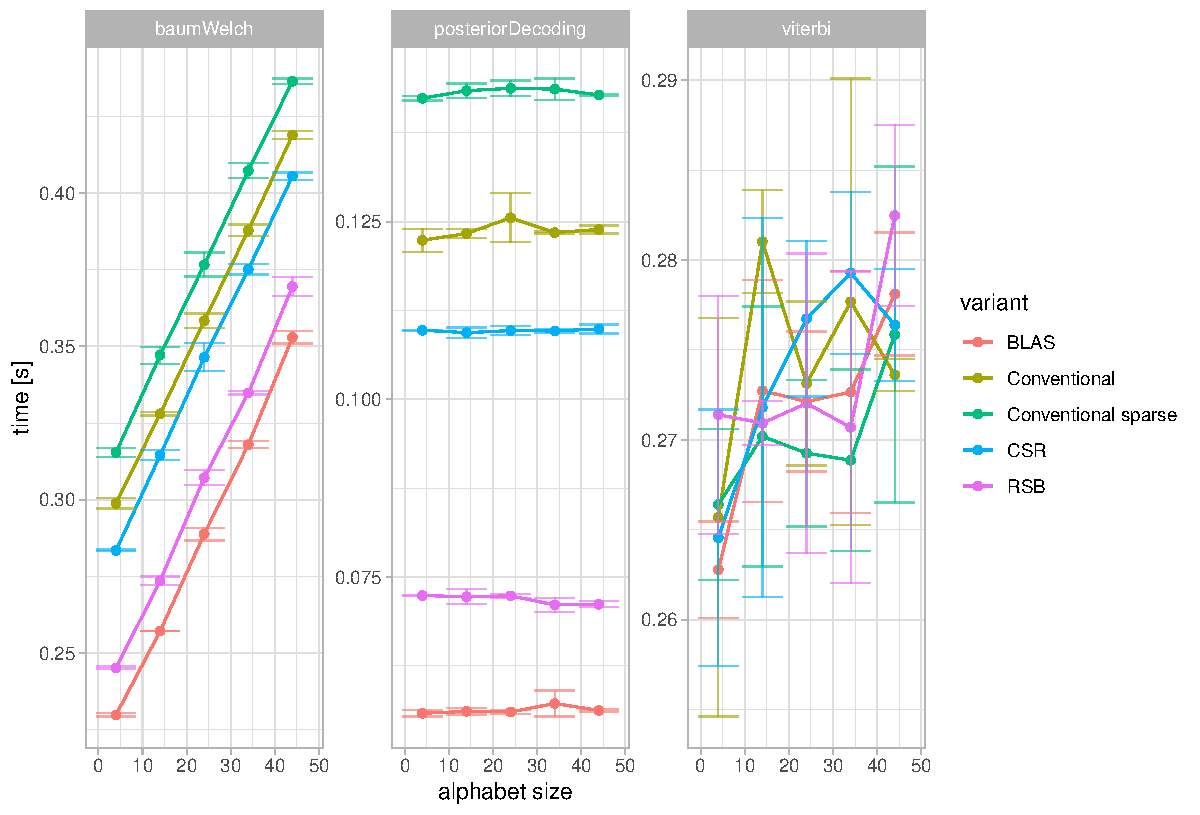
\includegraphics[scale=0.85]{figures/figure_C1.pdf}
%     \caption{Running time of increasing alphabet size for all implementations. All algorithms but Forward and Backward. Time measurement is averaged over 3 replicates. Error bars indicate standard deviation.}
%     \label{app:alphabet}
% \end{figure}


\begin{figure}[H]
    \centering
  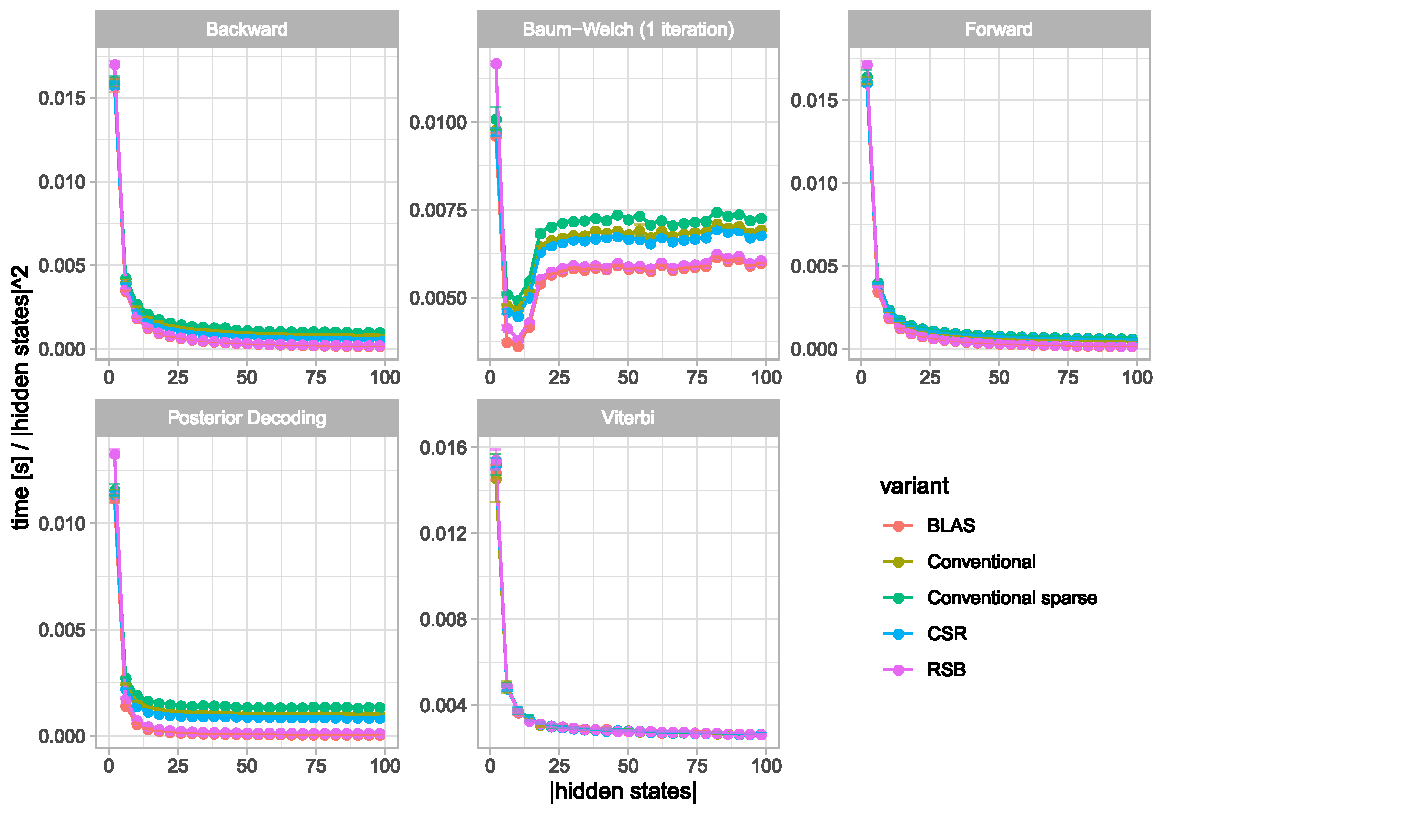
\includegraphics[scale=0.85]{figures/figure_C3_scaled.pdf}
    \caption{Running time of increasing number of hidden states for all algorithms and all implementations. Time measurement is averaged over 3 replicates. Error bars indicate standard deviation. Alphabet size = 4, input size = 100'000.}
    \label{app:hiddenstates}
\end{figure}




\begin{figure}[H]
    \centering
    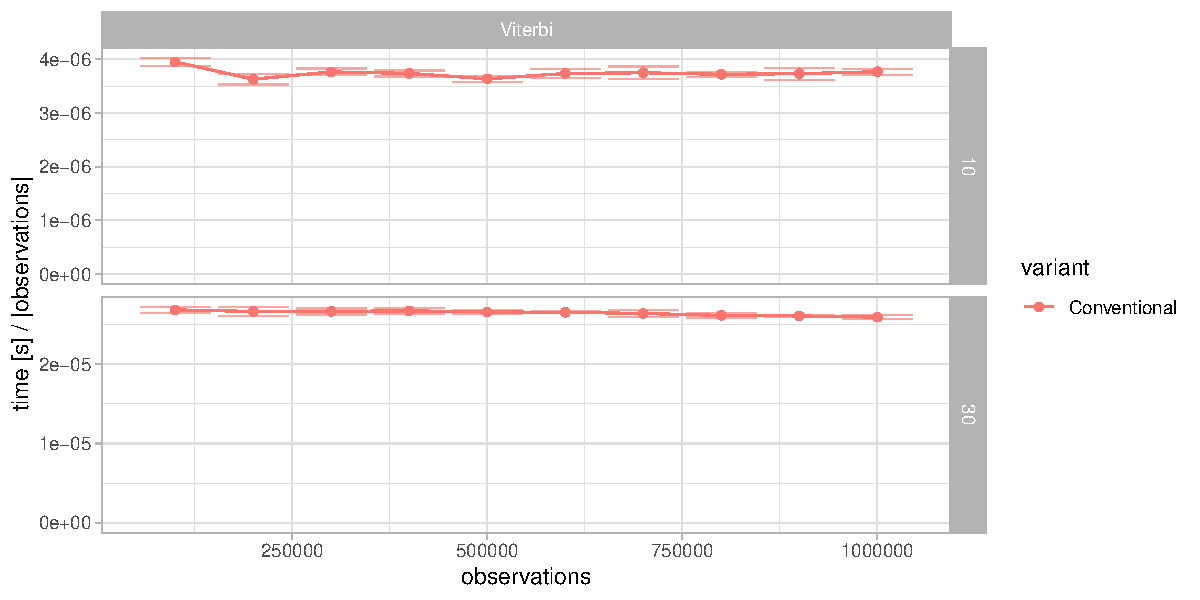
\includegraphics[scale=0.85]{figures/figure_A3_scaled.pdf}
    \caption{Running time of increasing number of observations in the Viterbi algorithm. For 10 and 30 hidden states. Time measurement is averaged over 3 replicates. Error bars indicate standard deviation. Alphabet size = 4. }
    \label{app:viterbi}
\end{figure}


%\begin{figure}[H]
%    \centering
%    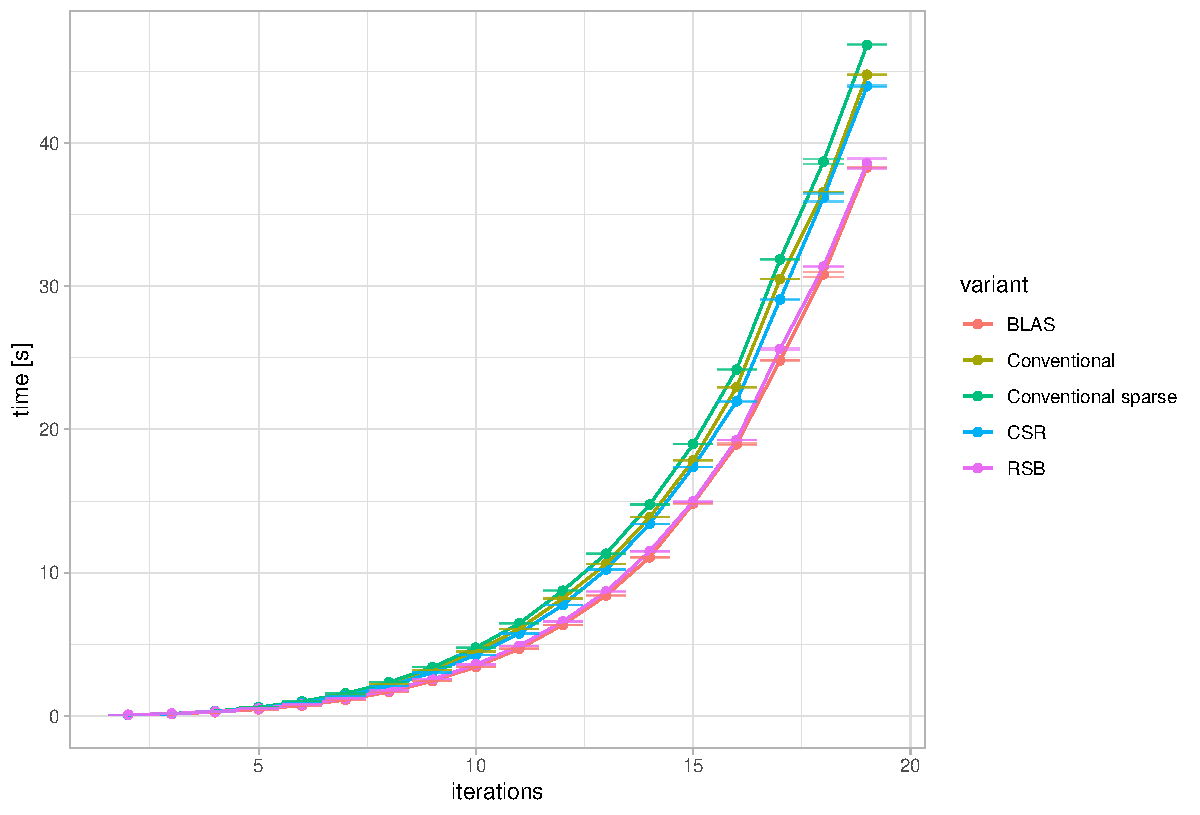
\includegraphics{figures/figure_C4_raw.pdf}
%    \caption{Running time for increasing iterations of the Baum-Welch algorithm. %Time measurement is averaged over 3 replicates. Error bars indicate standard %deviation. Alphabet size = 4, input size = 100'000 observations.}
%    \label{app:baumwelchiterations}
%\end{figure}
